\documentclass[11pt,a4paper]{article}
\usepackage[margin=2.4cm]{geometry}
\usepackage{amsmath,amssymb,bm}
\usepackage{graphicx}
\usepackage{booktabs}
\usepackage[numbers,sort&compress]{natbib}
\usepackage[colorlinks=true,linkcolor=blue!60!black,citecolor=blue!60!black,urlcolor=blue!60!black]{hyperref}
\usepackage{xcolor}
\IfFileExists{numbers.tex}{\newcommand{\chiStar}{3956}
\newcommand{\NcAct}{1.68\times10^{-7}}
\newcommand{\NcPl}{3.03\times10^{-7}}
\newcommand{\Cll}{2.78\times10^{-8}}
\newcommand{\Clc}{4.57\times10^{-8}}
\newcommand{\Ccc}{1.38\times10^{-7}}
\newcommand{\lmaxFifty}{1273}
\newcommand{\NFifty}{2.45\times10^{-8}}
\newcommand{\NbhFifty}{1.98\times10^{-7}}
\newcommand{\snrFiftyAct}{37}
\newcommand{\snrFiftyPl}{36}
\newcommand{\snrFiftyBhAct}{15}
}{}
% AAS journal macros used by ADS bibtex entries
\newcommand{\aap}{A\&A}\newcommand{\apj}{ApJ}\newcommand{\apjl}{ApJL}\newcommand{\apjs}{ApJS}
\newcommand{\mnras}{MNRAS}\newcommand{\prd}{Phys.\ Rev.\ D}\newcommand{\prl}{Phys.\ Rev.\ Lett.}
\newcommand{\jcap}{JCAP}\newcommand{\nat}{Nature}\newcommand{\aj}{AJ}\newcommand{\pasp}{PASP}
\newcommand{\araa}{ARA\&A}\newcommand{\physrep}{Phys.\ Rep.}\newcommand{\pasj}{PASJ}\newcommand{\apss}{Ap\&SS}

\newcommand{\dF}{\delta_F}
\newcommand{\dt}{\tilde\delta}
\newcommand{\vl}{\bm{l}}
\newcommand{\vL}{\bm{L}}
\newcommand{\vth}{\bm{\theta}}
\newcommand{\kpar}{k_\parallel}
\newcommand{\PP}{\mathcal{P}}
\newcommand{\dD}{\delta_{\rm D}}
\newcommand{\Tr}{\mathrm{Tr}}
\newcommand{\kcmb}{\kappa_{\rm CMB}}
\newcommand{\klya}{\kappa_{{\rm Ly}\alpha}}
\newcommand{\todo}[1]{\textcolor{red}{[#1]}}

\title{Weak lensing of the Lyman-$\alpha$ forest and its cross-correlation with CMB lensing:\\ literature review and the sample-variance-limited estimator}
\author{A.~Slosar, with Claude}
\date{Working notes, started 10 September 2026}

\begin{document}
\maketitle

\begin{abstract}
These notes accompany an attempt to detect gravitational lensing of the DESI DR1 Lyman-$\alpha$ forest through its cross-correlation with CMB lensing maps from ACT and Planck. Section~\ref{sec:lit} reviews the (small) literature on lensing of the forest and the adjacent literature on forest--CMB-lensing correlations and on lensing reconstruction from three-dimensional source fields. Section~\ref{sec:formalism} derives, in the flat-sky, single-source-plane, zero-noise (sample-variance) limit, the optimal quadratic estimator for the convergence from a set of forest pixels, the cubic estimator $W_{ijk}\dF^i\dF^j\kcmb^k$ for the cross-spectrum $C_L^{\klya\kcmb}$, its variance, the dense-sightline continuum limit with a closed-form reconstruction noise $N_\kappa(L)$, and a bias-hardened variant that projects out the response of the forest power spectrum to long-wavelength modes. Section~\ref{sec:numbers} evaluates $N_\kappa(L)$ and the cross-correlation signal-to-noise for a fiducial forest power spectrum and DESI-like sightline densities. The central qualitative result is that for sparse sightlines most of the naive sample-variance information comes from an isotropic dilation of the transverse correlation function that is degenerate with a local modulation of the forest power spectrum amplitude, and that the robust (shear-like) information is set by the transverse rather than the line-of-sight resolution.
\end{abstract}

\tableofcontents

\section{Literature review}
\label{sec:lit}

\subsection{Lensing of the forest}

Only one group has published on reconstructing the lensing potential from the forest itself.
\citet{1706.07870} proposed the idea: the three-dimensional forest is treated as a stack of source screens at $z\simeq2$--3 and a configuration-space quadratic estimator, adapted from 21\,cm lensing work, is applied to simulated spectra on a $15^\circ\times15^\circ$ field with a sightline every 1.8~arcmin (which they call the extreme high end of achievable densities). They recover the degree-scale morphology of the potential and give no per-survey signal-to-noise.
\citet{1706.08939} supplied Gaussian noise forecasts. The noise per potential mode scales as $\sigma_\tau^2/[j_{\max}(l_{\max}-l_{\min})^2l_{\min}^2]$, where $\sigma_\tau$ is the fractional per-pixel error and $j_{\max}$ the number of radial modes. Their cumulative signal-to-noise on the convergence power spectrum for DESI (770k spectra, 14\,000~deg$^2$, 8.1~arcmin mean separation, per-pixel S/N 3.3) is 7 for $\Delta z=0.1$ source bins and 29 for $\Delta z=0.5$ bins, corresponding to a 1.5 per cent measurement of the amplitude of mass fluctuations at $z\simeq2.5$; eBOSS gives 4--16 and an MSE-like survey 50--160.
\citet{2005.04109} replaced the harmonic estimator by a real-space minimum-variance pixel-pair estimator built on the full pixel covariance, with the potential expanded in Legendre polynomials over a patch. This handles irregular sightline positions, holes and inhomogeneous noise. On Gaussian mocks they find that high-fidelity maps require $\gtrsim0.5$ sources per arcmin$^2$ and signal-dominated pixels; a density of 200~deg$^{-2}$ fails.
\citet{2209.04564} applied that estimator to hydrodynamic simulations with ray-traced potentials: forest non-Gaussianity reduces the signal-to-noise by a factor of about 2.7 in the noise-free case and 1.5 for unit signal-to-noise spectra, and the recovered potential is biased by 5--25 per cent, which they correct by Gaussianizing the flux field.
\citet{2410.20014} forecast DESI directly: 50 quasars per deg$^2$, 700k spectra, pixel noise $\sigma_\delta=0.3$ after rebinning to 2.8~\AA\ and discarding the noisiest quarter, and detection defined as the correlation of the reconstructed potential with the foreground galaxy distribution. The full-survey significance is $S/N\simeq3$ (two-pixel estimator), 4 (four-pixel) and 9 without pixel noise; 200--2000~deg$^{-2}$ surveys on the same area reach 16--27. They state explicitly that they do not consider cross-correlation with CMB lensing.

No detection of forest lensing has been claimed, no analysis of eBOSS or DESI data exists, and no paper considers the cross-correlation of a forest-lensing reconstruction with CMB lensing. The last point is the gap this project targets: ACT DR6 \citep{2304.05202,2304.05203} and Planck PR4 \citep{2206.07773} lensing maps cover the full DESI DR1 forest footprint of more than 9500~deg$^2$ with 428\,403 valid Ly$\alpha$-region forests \citep{2404.03001}, and a cross-correlation is immune to the additive Gaussian ($N^{(0)}$-type) bias that dominates an auto-spectrum measurement.

\subsection{Forest--CMB-lensing correlations that are not lensing of the forest}

A separate line of work correlates the forest flux, or its local one-dimensional power, with $\kcmb$. \citet{0903.4171,0910.4125} forecast the two-point $\langle\dF\kcmb\rangle$ and the $\langle\dF^2\kcmb\rangle$ correlations; \citet{1607.03625} detected the latter at $5\sigma$ with BOSS DR12 and Planck 2015; \citet{1708.07512} modelled it as the squeezed gravitational bispectrum plus a term from mean-flux misestimation on finite skewers; \citet{2405.14988} detected it at $4.8\sigma$ with DESI Y1 forests and Planck PR3; \citet{2405.01628} forecast $S/N\simeq10$, 15 and 20 for DESI with ACT, Simons Observatory and CMB-S4. Physically these measure the response of the small-scale forest power to long-wavelength modes, quantified with separate-universe simulations by \citet{1701.03375}. This is important here for a negative reason: as shown in Section~\ref{sec:squeezed}, the same response mimics a lensing convergence in a quadratic estimator, so the detected $P_F\times\kcmb$ bispectrum is the leading contaminant of the measurement we want to make. \citet{1004.1165} discuss the related but distinct effect of quasar magnification bias on forest statistics, at the 0.1--1 per cent level.

\subsection{Lensing reconstruction from three-dimensional fields}

The formalism below follows the CMB quadratic estimator of \citet{astro-ph/0105424,astro-ph/0111606} generalized to a three-dimensional source by \citet{astro-ph/0511547}, who showed that each line-of-sight Fourier mode acts as an independent screen and that the screens combine with inverse-variance weights. \citet{0710.1108} pointed out that source non-Gaussianity sets a noise floor even without instrumental noise. \citet{1311.4484,1410.2533} developed the 21\,cm intensity-mapping version at $z\simeq2$--3 including discreteness noise. \citet{1803.04975} computed the bias to the three-dimensional estimator from the matter bispectrum, found it to cost a factor of a few in signal-to-noise for 21\,cm surveys, and introduced a bias-hardened estimator; \citet{1802.05706,1804.06403} generalized the estimator to weakly non-Gaussian sources and introduced the shear-only estimator that is immune to isotropic modulations of the source power. Bias hardening in the CMB context is due to \citet{1209.0091}; see also \citet{2007.04325,2101.12193}. \citet{2402.07988} recently applied the standard and shear-only estimators to projected galaxy clustering as the source, the closest analogue of a sparse-tracer reconstruction. A fuller annotated list is kept in \texttt{report/literature\_notes.md}.

\section{Formalism in the sample-variance limit}
\label{sec:formalism}

\subsection{Set-up and conventions}

We work in the flat-sky, distant-observer approximation. A point in the forest volume is labelled by an angular position $\vth$ (radians) and a comoving line-of-sight distance $\chi$; the effective comoving distance to the forest is $\chi_*$ ($\chi_*\simeq\chiStar\,h^{-1}$Mpc at $z=2.4$ for a Planck-2018 cosmology). The flux contrast $\dF(\vth,\chi)$ is treated as a statistically homogeneous Gaussian random field with the anisotropic (redshift-space) power spectrum $P_F(\kpar,k_\perp)$. Its Fourier transform in the mixed angular/radial variables is
\begin{equation}
\delta(\vl,\kpar)=\int d^2\theta\,d\chi\;\dF(\vth,\chi)\,e^{-i(\vl\cdot\vth+\kpar\chi)},\qquad
\langle\delta(\vl,\kpar)\delta(\vl',\kpar')\rangle=(2\pi)^3\dD^2(\vl+\vl')\dD(\kpar+\kpar')\,\PP(l,\kpar),
\label{eq:power}
\end{equation}
with $\PP(l,\kpar)=P_F(\kpar,k_\perp=l/\chi_*)/\chi_*^2$. Reality of $\dF$ implies $\delta(-\vl,-\kpar)=\delta^*(\vl,\kpar)$. For a survey of solid angle $\Omega$ and radial depth $D$ the coincident delta functions are $(2\pi)^2\dD^2(0)=\Omega$ and $2\pi\dD(0)=D$.

Lensing by a single effective source plane at $\chi_s$ is described by a projected potential $\phi(\vth)$ with deflection $\bm\alpha=\nabla\phi$, convergence $\kappa=-\nabla^2\phi/2$ (so $\kappa(\vL)=L^2\phi(\vL)/2$) and shear $\gamma_1=-(\partial_1^2-\partial_2^2)\phi/2$, $\gamma_2=-\partial_1\partial_2\phi$, exactly the convention of \citet{astro-ph/0111606}. The observed forest field is
\begin{equation}
\dt(\vth,\chi)=\dF\big(\vth+\nabla\phi(\vth),\chi\big).
\label{eq:lensed}
\end{equation}
Because the source plane is common to all $\chi$, the displacement is independent of the radial coordinate; this is the single approximation that makes the problem separable in $\kpar$. In reality the lensing kernel changes by a few per cent across a forest, which we defer to later work.

\subsection{Mode coupling induced by lensing}
\label{sec:coupling}

Expanding \eqref{eq:lensed} to first order, $\dt=\dF+\nabla\phi\cdot\nabla_\theta\dF$, and Fourier transforming,
\begin{equation}
\dt(\vl,\kpar)=\delta(\vl,\kpar)-\int\frac{d^2l_1}{(2\pi)^2}\,\big[\vl_1\cdot(\vl-\vl_1)\big]\,\phi(\vl-\vl_1)\,\delta(\vl_1,\kpar).
\label{eq:dt}
\end{equation}
For a fixed realization of $\phi$ the two-point function of the observed field acquires an off-diagonal part. With $\vL=\vl+\vl'$ and $\vL\neq0$,
\begin{equation}
\big\langle\dt(\vl,\kpar)\,\dt(\vl',\kpar')\big\rangle_\phi
=2\pi\dD(\kpar+\kpar')\Big[(2\pi)^2\dD^2(\vL)\PP(l,\kpar)+f(\vl,\vl';\kpar)\,\phi(\vL)\Big],
\qquad
f(\vl,\vl';\kpar)=\vL\cdot\vl\,\PP(l,\kpar)+\vL\cdot\vl'\,\PP(l',\kpar).
\label{eq:coupling}
\end{equation}
It is convenient to express the response in terms of the convergence, $f_\kappa\equiv 2f/L^2$, so that the off-diagonal term reads $f_\kappa\,\kappa(\vL)$. Equation~\eqref{eq:coupling} is diagonal in $\kpar$: every radial Fourier mode is an independently lensed two-dimensional screen with power spectrum $\PP(l,\kpar)$, all sharing the same $\phi$ \citep{astro-ph/0511547}. Pairs with $\kpar'\neq-\kpar$ carry no lensing information and, for a Gaussian field, no covariance either, so an optimal estimator never uses them.

\paragraph{The pair-displacement picture.}
The same result follows from the real-space statement in the task description: a pair of pixels $i=(a,p)$ and $j=(b,q)$ on sightlines $a,b$ at radial positions $\chi_p,\chi_q$ has covariance
\begin{equation}
C_{ij}(\phi)=\xi\big(\vth_{ab}+\bm\alpha_a-\bm\alpha_b,\ \chi_p-\chi_q\big)
\simeq \xi(\vth_{ab},\Delta\chi_{pq})+\nabla_\theta\xi(\vth_{ab},\Delta\chi_{pq})\cdot\big[\nabla\phi(\vth_a)-\nabla\phi(\vth_b)\big],
\label{eq:pair}
\end{equation}
where $\xi$ is the correlation function of $\dF$ in angular--radial coordinates and $\vth_{ab}=\vth_a-\vth_b$. Only the relative deflection of the two members of a pair matters, so a pair measures the local tidal field of $\phi$ rather than the deflection itself. Fourier transforming \eqref{eq:pair} over both positions reproduces \eqref{eq:coupling}; this was verified symbolically for a periodic one-dimensional toy model in \texttt{mathematica/pair\_displacement\_check.wls}.

\subsection{Squeezed limit: dilation, shear and the amplitude degeneracy}
\label{sec:squeezed}

For lens modes much larger than the forest modes, $L\ll l$, expanding \eqref{eq:coupling} to second order in $L$ gives (verified in \texttt{mathematica/lensing\_response\_checks.wls}, check A)
\begin{equation}
f_\kappa(\vl,\vL-\vl)\simeq 2\PP(l)+2\,(\hat{\vL}\cdot\hat{\vl})^2\,l\,\PP'(l)
=\underbrace{\big[2\PP+l\PP'\big]}_{\text{dilation}}+\underbrace{l\PP'\cos2\varphi_{lL}}_{\text{shear}},
\label{eq:squeezed}
\end{equation}
with $\PP'=\partial\PP/\partial l$ at fixed $\kpar$. The two pieces have a clean geometric meaning. For a pair separation $\theta_{ab}$ small compared with the lens wavelength, $\bm\alpha_a-\bm\alpha_b\simeq(\vth_{ab}\cdot\nabla)\nabla\phi=-(\kappa\,\mathbb{1}+\bm\gamma)\vth_{ab}$, so the pair correlation is evaluated at the true separation $(1-\kappa)\vth_{ab}-\bm\gamma\vth_{ab}$: the convergence isotropically dilates the transverse correlation function while the shear makes it anisotropic. In Fourier space the exact power spectrum of a field dilated and sheared by constant $\kappa,\gamma_1,\gamma_2$ is $\PP(|M^{-T}\vl|)/\det M$ with $M=\mathbb{1}-\kappa\mathbb{1}-\bm\gamma$, whose first-order expansion equals \eqref{eq:squeezed} (check B in the same script).

The amplitude degeneracy is now apparent. A slowly varying multiplicative modulation of the field, $\dt=(1+a)\dF$, produces the coupling
\begin{equation}
\big\langle\dt(\vl,\kpar)\dt(\vl',\kpar')\big\rangle\supset 2\pi\dD(\kpar+\kpar')\,f_a(\vl,\vl';\kpar)\,a(\vL),\qquad f_a=\PP(l,\kpar)+\PP(l',\kpar)\xrightarrow{L\ll l}2\PP,
\label{eq:famp}
\end{equation}
so the dilation term $2\PP+l\PP'=(2+n)\PP$, with $n=d\ln\PP/d\ln l$, is proportional to the amplitude response. For a transverse spectrum that is locally a power law the convergence is therefore \emph{indistinguishable} from a local change of the forest power spectrum amplitude by $\delta\ln P_F=(2+n)\kappa$; only the shear term $l\PP'\cos2\varphi$ and departures from a power law break the degeneracy. For $n=-2$ the dilation response vanishes identically, and for a spectrum that is flat in $l$ ($n=0$, which is what the forest looks like transversely whenever $l/\chi_*\ll\kpar$) there is no shear response at all and the entire lensing signal is an amplitude change. This matters because the forest power spectrum really is modulated by long-wavelength density and tidal modes, with responses measured by \citet{1701.03375}, and those long modes are correlated with $\kcmb$. That correlation is exactly the $P_F\times\kcmb$ bispectrum detected by \citet{1607.03625,2405.14988}, and it will enter our cubic estimator as an additive bias unless projected out (Section~\ref{sec:hardening}).

\subsection{The optimal quadratic estimator for discrete pixels}
\label{sec:discrete}

Let $d_i=\dt(\vth_{a(i)},\chi_{p(i)})$, $i=1\dots N_{\rm pix}$, be the vector of all forest pixels on all sightlines, in the zero-noise limit. Expand the potential in a set of real basis functions, $\phi(\vth)=\sum_\mu p_\mu\psi_\mu(\vth)$; in the continuum limit below the $\psi_\mu$ are Fourier modes, while on a finite irregular footprint one may use Legendre or Zernike polynomials as in \citet{2005.04109}. To first order in $p$ the pixel covariance is, from \eqref{eq:pair},
\begin{equation}
C_{ij}(p)=C^0_{ij}+\sum_\mu p_\mu\,C^{,\mu}_{ij},\qquad
C^{,\mu}_{ij}=\nabla_\theta\xi(\vth_{ab},\Delta\chi_{pq})\cdot\big[\nabla\psi_\mu(\vth_a)-\nabla\psi_\mu(\vth_b)\big].
\label{eq:Cderiv}
\end{equation}
For a Gaussian likelihood $-2\ln\mathcal L=d^TC^{-1}d+\ln\det C$ the Newton--Raphson step from $p=0$ is the optimal (minimum-variance, unbiased to first order) quadratic estimator,
\begin{equation}
\hat p_\mu=\tfrac12\sum_\nu F^{-1}_{\mu\nu}\Big[d^TC_0^{-1}C^{,\nu}C_0^{-1}d-\Tr\big(C_0^{-1}C^{,\nu}\big)\Big],
\qquad
F_{\mu\nu}=\tfrac12\Tr\big(C_0^{-1}C^{,\mu}C_0^{-1}C^{,\nu}\big).
\label{eq:qe}
\end{equation}
Writing $\hat p_\mu=\sum_{ij}E^\mu_{ij}d_id_j-b_\mu$ identifies the quadratic weights and the mean field,
\begin{equation}
E^\mu=\tfrac12\sum_\nu F^{-1}_{\mu\nu}\,C_0^{-1}C^{,\nu}C_0^{-1},\qquad b_\mu=\sum_{ij}E^\mu_{ij}C^0_{ij}.
\label{eq:E}
\end{equation}
Using $\langle d_id_j\rangle=C_{ij}(p)$ one checks $\langle\hat p_\mu\rangle=p_\mu+O(p^2)$, and for Gaussian $d$ the covariance at $p=0$ is $\mathrm{Cov}(\hat p_\mu,\hat p_\nu)=F^{-1}_{\mu\nu}$, which saturates the Cram\'er--Rao bound. The convergence coefficients follow by applying $-\nabla^2/2$ to the basis; for Fourier modes $\hat\kappa_{\vL}=(L^2/2)\hat\phi_{\vL}$. Two remarks. First, the same formulae hold with pixel noise by replacing $C^0\to C^0+N$, so nothing in this section is specific to the sample-variance limit except the numerical value of $F$. Second, because $E^\mu$ is built from ratios of $C^0$ and its derivative, an overall rescaling of the forest power spectrum leaves the estimator and its variance unchanged: in the zero-noise limit the reconstruction noise depends only on the \emph{shape} of $P_F$ and on the geometry of the pixel set.

\subsection{The cubic cross-correlation estimator}
\label{sec:cubic}

Let $m_k$ be the pixels of a CMB convergence map and $\kappa^{\rm CMB}_{\vL}=\sum_kY_{\vL k}m_k$ its (masked, apodized) flat-sky harmonic transform, normalized so that $\langle\kappa_{\vL}\kappa^*_{\vL'}\rangle=\Omega\,\delta_{\vL\vL'}C_L$ for a full-sky-normalized spectrum. Choosing Fourier modes as the basis in \eqref{eq:qe}, the natural bandpower estimator for the cross-spectrum in a bin $b$ containing $N_b$ modes is
\begin{equation}
\hat C_b=\frac{1}{\Omega N_b}\sum_{\vL\in b}\mathrm{Re}\big[\hat\kappa_{\vL}\,\kappa^{{\rm CMB}*}_{\vL}\big]
=\sum_{ijk}W^b_{ijk}\,d_id_jm_k-\frac{1}{\Omega N_b}\sum_{\vL\in b}\mathrm{Re}\big[b_{\vL}\kappa^{{\rm CMB}*}_{\vL}\big],
\qquad
W^b_{ijk}=\frac{1}{\Omega N_b}\sum_{\vL\in b}\mathrm{Re}\big[E^{\vL}_{ij}Y^*_{\vL k}\big].
\label{eq:cubic}
\end{equation}
This is the cubic form $W_{ijk}\dF^i\dF^j\kcmb^k$ anticipated in the task description, with the weights fixed by \eqref{eq:E}. Its properties:
\begin{itemize}
\item \textbf{Expectation.} To first order in $\phi$, $\langle\hat C_b\rangle=\bar C_b^{\klya\kcmb}$, the bin average of the true cross-spectrum. The mean-field term is a fixed function of the pixel geometry and is uncorrelated with $\kcmb$, so it averages to zero but should be subtracted to avoid excess variance.
\item \textbf{No Gaussian ($N^{(0)}$) bias.} The disconnected part of $\langle d_id_jm_k\rangle$ vanishes because $\langle m_k\rangle=0$ and the Gaussian part of $d_id_j$ is independent of $m_k$. This is the main advantage of the cross-correlation over the auto-spectrum of $\hat\kappa$, whose $N^{(0)}$ bias equals the full reconstruction noise.
\item \textbf{Second-order lensing ($N^{(1)}$-type) bias.} At $O(\phi^2)$, contracting $\kcmb$ with one power of $\phi$ and the remaining $\phi$ with the two $\dF$ fields gives a term proportional to $\int d^2L'\,C_{L'}^{\klya\kcmb}\times(\text{coupling kernel})$, the analogue of the CMB $N^{(1)}$ bias. It is a few-per-cent correction that must be computed with the fiducial spectra.
\item \textbf{Intrinsic clustering bias.} $\dF$ is itself a biased tracer of the matter at $z\simeq2$--3, which lies inside the CMB lensing kernel. The connected bispectrum $\langle\dF\dF\kcmb\rangle_c$ therefore contributes even in the absence of lensing of the forest. Its squeezed part is the response of $P_F$ to long modes, $\delta\ln P_F=R_\delta\,\delta_L+R_K\,K_L$ (density and tidal responses), correlated with $\kcmb$; in the language of Section~\ref{sec:squeezed} it enters as $\langle\hat a_{\vL}\kappa^{{\rm CMB}*}_{\vL}\rangle\neq0$ projected onto $\hat\kappa$ through the response ratio $F_{\kappa a}/F_{\kappa\kappa}$. This is the forest analogue of the gravitational-nonlinearity bias of \citet{1803.04975} and it is not small: it is the signal that \citet{2405.14988} detected at $4.8\sigma$ in DESI Y1.
\item \textbf{Variance.} For Gaussian fields and optimal weights the variance in the continuum limit is
\begin{equation}
\mathrm{Var}(\hat C_b)=\frac{\big(C_L^{\klya\klya}+N_\kappa(L)\big)\big(C_L^{\kcmb\kcmb}+N_L^{\rm CMB}\big)+\big(C_L^{\klya\kcmb}\big)^2}{f_{\rm sky}(2L+1)\Delta L},
\label{eq:var}
\end{equation}
with $N_\kappa(L)$ the reconstruction noise derived next. For a general pixel set the numerator's first factor is replaced by the appropriate combination of $F^{-1}$, i.e. by $\mathrm{Cov}(\hat\kappa_{\vL},\hat\kappa_{\vL'})$ from \eqref{eq:qe}.
\end{itemize}

\subsection{Continuum limit: Hu--Okamoto form and reconstruction noise}
\label{sec:continuum}

For infinitely dense sightlines and complete radial coverage over a depth $D$, the field is measured on a regular three-dimensional grid and the Fisher matrix of Fourier modes becomes diagonal. It is then simpler to derive the estimator directly. Take
\begin{equation}
\hat\kappa(\vL)=A(L)\int\frac{d\kpar}{2\pi}\int\frac{d^2l}{(2\pi)^2}\,g(\vl,\vL-\vl;\kpar)\,\dt(\vl,\kpar)\,\dt(\vL-\vl,-\kpar).
\label{eq:HO}
\end{equation}
Inserting \eqref{eq:coupling}, the coincident radial delta function gives $2\pi\dD(0)=D$, so $\langle\hat\kappa(\vL)\rangle=\kappa(\vL)$ requires
\begin{equation}
A(L)^{-1}=D\int\frac{d\kpar}{2\pi}\int\frac{d^2l}{(2\pi)^2}\,g\,f_\kappa .
\end{equation}
The Gaussian variance of \eqref{eq:HO} at $\phi=0$ has two Wick pairings, each producing another factor $D$ and the power spectra of the two legs; minimizing it subject to the normalization gives the standard weight $g=f_\kappa/[2\PP(l,\kpar)\PP(|\vL-\vl|,\kpar)]$ and
\begin{equation}
\boxed{\;
\frac{1}{N_\kappa(L)}=D\int_{-\infty}^{\infty}\frac{d\kpar}{2\pi}\;I_{\kappa\kappa}(L,\kpar),\qquad
I_{XY}(L,\kpar)=\int\frac{d^2l}{(2\pi)^2}\,\frac{f_X(\vl,\vL-\vl;\kpar)\,f_Y(\vl,\vL-\vl;\kpar)}{2\,\PP(l,\kpar)\,\PP(|\vL-\vl|,\kpar)}\;}
\label{eq:Nkappa}
\end{equation}
with $\langle\hat\kappa(\vL)\hat\kappa^*(\vL')\rangle=(2\pi)^2\dD^2(\vL-\vL')[C_L^{\kappa\kappa}+N_\kappa(L)]$. Equation~\eqref{eq:Nkappa} is the inverse-variance sum over independent $\kpar$ screens of the Hu--Okamoto noise of each screen, $N_{\kpar}^{-1}=I_{\kappa\kappa}$, with the mode density $D\,d\kpar/2\pi$ counting the screens \citep{astro-ph/0511547}. It is the same object as $F^{-1}$ of \eqref{eq:qe} per unit solid angle. Two consistency checks: (i) since $f_\kappa\propto\PP$, the integrand is invariant under $\PP\to c\PP$, as it must be in the sample-variance limit; (ii) for a white spectrum, $\PP=$ const, $f_\kappa=2\PP$ exactly, so $I_{\kappa\kappa}=l_{\max}^2/2\pi$ and $N_\kappa^{-1}=Dk_{\max}l_{\max}^2/2\pi^2$; this equals twice the number of real degrees of freedom per steradian of the field, which is what one obtains directly by noting that a dilation by $\kappa$ changes the variance of every independent white-noise pixel by a factor $(1+2\kappa)$ and each pixel then carries Fisher information $\frac12(2)^2=2$. The numerical implementation (\texttt{code/recon\_noise.py}) reproduces this count to the accuracy of the $|\vL-\vl|\le l_{\max}$ edge exclusion.

The cutoffs $l_{\max}$ and $k_{\parallel,\max}$ are where the real survey enters even in this idealization: transverse modes are only measured up to the sightline Nyquist frequency, $l_{\max}\simeq\pi/\bar\theta_{\rm sep}=\pi\sqrt{n_q}$ for $n_q$ sightlines per steradian, radial modes up to a fraction of the pixel Nyquist frequency, and radial modes below $k_{\parallel,\min}\sim0.03\,h\,{\rm Mpc}^{-1}$ are removed by continuum fitting. With sightlines of mean forest length $D_f$ covering only part of the total depth, the product $D\,l_{\max}^2$ that controls \eqref{eq:Nkappa} is fixed by the total sightline length per unit area, so one may use $D=D_f$ together with the full $n_q$. Sparse sampling also aliases small-scale transverse power into the measured band; that effect is beyond the continuum treatment and is one reason the numbers below are optimistic.

\subsection{Hardening against amplitude modulation}
\label{sec:hardening}

An estimator $\hat a(\vL)$ for the amplitude modulation is built from \eqref{eq:HO} with $f_a$ in place of $f_\kappa$, and the two estimators respond to each other's field with response functions $R_{\kappa a}(L)=F_{\kappa a}/F_{\kappa\kappa}$ and $R_{a\kappa}=F_{\kappa a}/F_{aa}$, where $F_{XY}=D\int d\kpar/2\pi\,I_{XY}$. The bias-hardened estimator \citep{1209.0091}
\begin{equation}
\hat\kappa^{\rm BH}=\frac{\hat\kappa-R_{\kappa a}\hat a}{1-R_{\kappa a}R_{a\kappa}},\qquad
N^{\rm BH}_\kappa(L)=\frac{N_\kappa(L)}{1-\rho^2_{\kappa a}(L)},\qquad
\rho^2_{\kappa a}=\frac{F_{\kappa a}^2}{F_{\kappa\kappa}F_{aa}},
\label{eq:BH}
\end{equation}
has zero response to any $a(\vth)$ that multiplies all $\kpar$ modes equally. Since the true responses $R_\delta(\kpar,k_\perp)$ of the forest are scale dependent, a more conservative choice hardens each $\kpar$ screen separately, $1/N^{\rm BH,slice}_\kappa=D\int d\kpar/2\pi\,I_{\kappa\kappa}(1-\rho^2_{\kappa a}(L,\kpar))$; this removes any modulation of the form $a(\vth,\kpar)$ and keeps only the information that is genuinely anisotropic or shape-changing within a screen. Both variants are evaluated below; the truth for the real forest lies in between and also requires hardening against the tidal response, which mimics shear rather than convergence and would need the $k_\perp$-dependence of $R_K$ to be separated from $l\PP'$.

\subsection{The signal and its detectability}
\label{sec:signal}

In the Limber approximation, with a single forest source plane at $\chi_*$ and the CMB at $\chi_{\rm CMB}$,
\begin{equation}
C_L^{XY}=\int_0^{\chi_{\min}}d\chi\,\frac{W_X(\chi)W_Y(\chi)}{\chi^2}\,P_{\rm m}\!\Big(k=\frac{L+1/2}{\chi},z(\chi)\Big),\qquad
W_s(\chi)=\frac32\Omega_{\rm m}\Big(\frac{H_0}{c}\Big)^2(1+z)\,\chi\,\frac{\chi_s-\chi}{\chi_s},
\label{eq:limber}
\end{equation}
and the total detection significance of the cross-spectrum from \eqref{eq:var} is
\begin{equation}
\Big(\frac{S}{N}\Big)^2=\sum_L f_{\rm sky}(2L+1)\,\frac{\big(C_L^{\klya\kcmb}\big)^2}{\big(C_L^{\klya\klya}+N_\kappa(L)\big)\big(C_L^{\kcmb\kcmb}+N_L^{\rm CMB}\big)+\big(C_L^{\klya\kcmb}\big)^2}.
\label{eq:snr}
\end{equation}
Because the forest source plane sits well inside the CMB lensing kernel the two convergences are strongly correlated, with $r_L=C^{\klya\kcmb}_L/(C^{\klya\klya}_LC^{\kcmb\kcmb}_L)^{1/2}\simeq0.9$ at $L=10$ falling to $0.67$ at $L\gtrsim300$.

\section{Toy numbers}
\label{sec:numbers}

\paragraph{Fiducial model.}
The forest power spectrum is the Kaiser form with the non-linear correction of \citet{1506.04519}, $P_F=b_F^2(1+\beta_F\mu^2)^2P_{\rm lin}(k)\,D_{\rm NL}(k,\mu)$, with approximate $z=2.4$ parameters $b_F=-0.13$, $\beta_F=1.6$, $q_1=0.6$, $q_2=0$, $k_v=1\,h\,{\rm Mpc}^{-1}$, $a_v=0.55$, $b_v=1.6$, $k_p=16\,h\,{\rm Mpc}^{-1}$ (\texttt{code/forest\_power.py}; only the shape matters here). The linear and non-linear matter power spectra come from CAMB for a Planck-2018 cosmology. The radial depth is $D=350\,h^{-1}$Mpc (one forest), the radial band is $0.03\le\kpar\le k_{\parallel,\max}$ with $k_{\parallel,\max}\in\{1,2,5\}\,h\,{\rm Mpc}^{-1}$, and the transverse cutoff is the sightline Nyquist multipole for $n_q\in\{20,50,100,400\}$~deg$^{-2}$ ($l_{\max}=\lmaxFifty$ for the DESI-DR1-like value $n_q=50$; DR1 has about 45 forests per deg$^2$ over 9500~deg$^2$). Figure~\ref{fig:pf} shows the fiducial spectrum.

\begin{figure}
\centering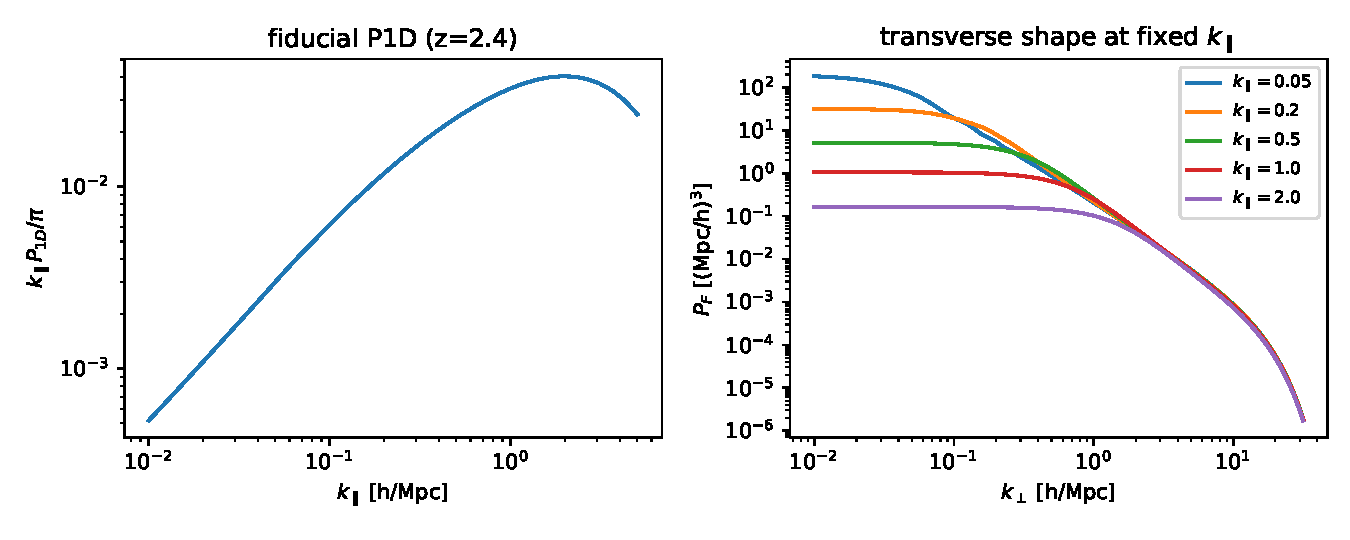
\includegraphics[width=0.95\textwidth]{figures/forest_power.pdf}
\caption{Fiducial forest power spectrum at $z=2.4$. Left: the implied one-dimensional power. Right: the transverse shape at fixed $\kpar$; for $k_\perp\ll\kpar$ the spectrum is flat in $l$, which is the regime in which lensing is degenerate with an amplitude change (Section~\ref{sec:squeezed}).}
\label{fig:pf}
\end{figure}

\paragraph{CMB lensing noise.}
Rather than fabricate noise curves, we use white noise levels calibrated to reproduce the published detection significances of the auto-spectra: $N_L^{\rm CMB}=\NcAct$ reproduces $43\sigma$ over $40\le L\le763$ on $f_{\rm sky}=0.23$ for ACT DR6 \citep{2304.05202}, and $N_L^{\rm CMB}=\NcPl$ reproduces the $\simeq42\sigma$-equivalent amplitude error over $8\le L\le400$ on $f_{\rm sky}=0.67$ for Planck PR4 \citep{2206.07773}. Real noise curves rise steeply at high $L$ and should replace these before any forecast is quoted externally. Overlap fractions of $f_{\rm sky}=0.15$ (ACT) and $0.22$ (Planck, the full DESI DR1 forest area) are assumed.

\paragraph{Results.}
Figure~\ref{fig:noise} compares $N_\kappa(L)$ with the signal spectra and Table~\ref{tab:numbers} lists values at $L=100$, where $C_{100}^{\klya\klya}=\Cll$, $C_{100}^{\klya\kcmb}=\Clc$ and $C_{100}^{\kcmb\kcmb}=\Ccc$.

\begin{figure}
\centering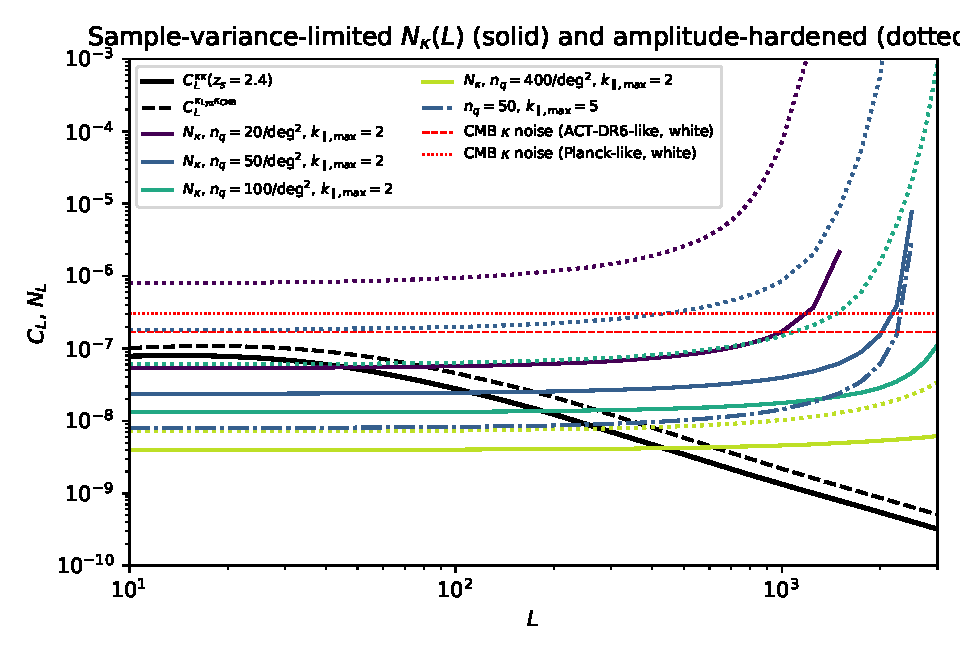
\includegraphics[width=0.8\textwidth]{figures/recon_noise.pdf}
\caption{Sample-variance-limited reconstruction noise $N_\kappa(L)$ (solid, Eq.~\ref{eq:Nkappa}) for sightline densities $n_q$ and $k_{\parallel,\max}=2\,h\,{\rm Mpc}^{-1}$, its per-screen amplitude-hardened version (dotted, Eq.~\ref{eq:BH}), and the case $k_{\parallel,\max}=5$ for $n_q=50$ (dash-dotted). Black curves are the forest convergence auto-spectrum and its cross-spectrum with $\kcmb$; red lines are the white-noise equivalents of the ACT DR6 and Planck PR4 reconstruction noise.}
\label{fig:noise}
\end{figure}

\begin{table}
\centering\small
\caption{Reconstruction noise at $L=100$ and cumulative cross-correlation signal-to-noise (to $L=3000$) in the sample-variance limit. $N^{\rm BH}$ is the per-screen amplitude-hardened noise. S/N columns are for $k_{\parallel,\max}=2$; the last column uses $N^{\rm BH}$ with ACT-like CMB noise.}
\label{tab:numbers}
\begin{tabular}{rrrccrrr}
\toprule
$n_q$ [deg$^{-2}$] & $l_{\max}$ & $k_{\parallel,\max}$ & $N_\kappa(100)$ & $N_\kappa^{\rm BH}(100)$ & S/N ACT & S/N Planck & S/N ACT, BH\\
\midrule
20 & 805 & 1.0 & $1.36\times10^{-7}$ & $9.49\times10^{-7}$ &  &  &  \\
 &  & 2.0 & $5.71\times10^{-8}$ & $9.44\times10^{-7}$ & 25.7 & 25.4 & 7.1 \\
 &  & 5.0 & $2.04\times10^{-8}$ & $9.43\times10^{-7}$ &  &  &  \\
50 & 1273 & 1.0 & $6.21\times10^{-8}$ & $2.01\times10^{-7}$ &  &  &  \\
 &  & 2.0 & $2.45\times10^{-8}$ & $1.98\times10^{-7}$ & 36.5 & 35.7 & 15.2 \\
 &  & 5.0 & $8.27\times10^{-9}$ & $1.97\times10^{-7}$ &  &  &  \\
100 & 1800 & 1.0 & $3.40\times10^{-8}$ & $6.63\times10^{-8}$ &  &  &  \\
 &  & 2.0 & $1.33\times10^{-8}$ & $6.37\times10^{-8}$ & 46.1 & 44.6 & 25.0 \\
 &  & 5.0 & $4.26\times10^{-9}$ & $6.32\times10^{-8}$ &  &  &  \\
400 & 3600 & 1.0 & $8.15\times10^{-9}$ & $8.84\times10^{-9}$ &  &  &  \\
 &  & 2.0 & $4.01\times10^{-9}$ & $7.33\times10^{-9}$ & 67.4 & 64.2 & 54.4 \\
 &  & 5.0 & $1.21\times10^{-9}$ & $7.05\times10^{-9}$ &  &  &  \\
\bottomrule
\end{tabular}

\end{table}

\begin{figure}
\centering
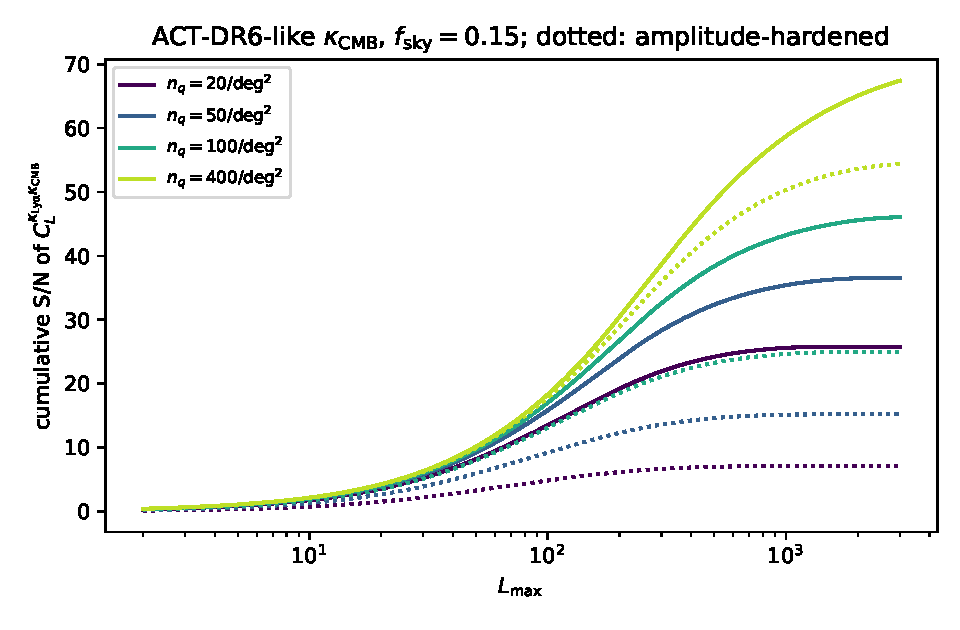
\includegraphics[width=0.48\textwidth]{figures/cross_snr.pdf}\hfill
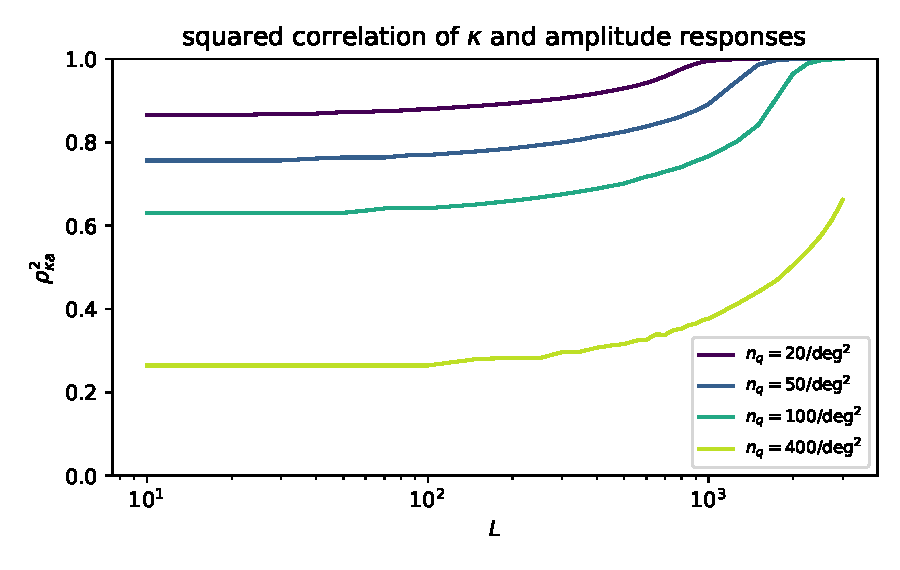
\includegraphics[width=0.48\textwidth]{figures/rho2.pdf}
\caption{Left: cumulative signal-to-noise of $C_L^{\klya\kcmb}$ for ACT-like CMB noise and $f_{\rm sky}=0.15$, with (dotted) and without (solid) amplitude hardening. Right: squared correlation coefficient between the convergence and amplitude responses, $\rho^2_{\kappa a}$ of Eq.~\eqref{eq:BH}, after summing over $\kpar$ screens.}
\label{fig:snr}
\end{figure}

Three features of these numbers are robust even though their absolute values are not:
\begin{enumerate}
\item For a DESI-like density the naive sample-variance noise at $L\sim100$, $N_\kappa=\NFifty$, is comparable to the signal $C_L^{\klya\klya}$, and it falls steeply with $k_{\parallel,\max}$ (as $1/k_{\parallel,\max}$ when the transverse spectrum is flat) and with $n_q$ (as $1/l_{\max}^2\propto1/n_q$).
\item The amplitude-hardened noise is $\sim8$ times larger for $n_q=50$ ($N^{\rm BH}_\kappa=\NbhFifty$), $\sim17$ times larger for $n_q=20$, and it is almost independent of $k_{\parallel,\max}$. This is the quantitative form of Section~\ref{sec:squeezed}: radial modes with $\kpar\gg l_{\max}/\chi_*$ see a transversely flat spectrum, and for them lensing is purely an amplitude change. The information that survives hardening comes from the few screens with $\kpar\lesssim l_{\max}/\chi_*\simeq0.3\,h\,{\rm Mpc}^{-1}$, so it is set by the sightline density alone. Increasing the density from 50 to 400~deg$^{-2}$ reduces $N^{\rm BH}_\kappa$ by a factor $\sim30$, faster than the $n_q^{-1}$ scaling of the naive noise, because it also converts amplitude-degenerate modes into shear-sensitive ones.
\item With ACT-like CMB noise the sample-variance-limited cross-correlation would be detected at $\simeq\snrFiftyAct\sigma$ for $n_q=50$ (Planck: $\snrFiftyPl\sigma$), dominated by $L\lesssim500$. These numbers are upper limits of no practical relevance by themselves: DESI pixel noise ($\sigma_\delta\simeq0.8$ per 0.8~\AA\ pixel against a forest rms of 0.34) removes most radial modes above $\kpar\sim0.5\,h\,{\rm Mpc}^{-1}$, sparse sampling aliases transverse power, and the estimator's own $N^{(1)}$ and clustering biases are not included. \citet{2410.20014} find $S/N\simeq3$--4 for the reconstructed potential against foreground galaxies with realistic noise. The route from the numbers here to a realistic forecast is to add the pixel noise to $\PP$ in \eqref{eq:Nkappa}, treat the sightline sampling explicitly through \eqref{eq:qe}, and compute the bias terms.
\end{enumerate}

\section{Caveats and next steps}

\begin{itemize}
\item \textbf{Single source plane.} Pixels at different $\chi$ are lensed by slightly different convergences; the estimator as written recovers a $\kpar$-weighted average. Modelling this is straightforward within \eqref{eq:qe} (each screen gets its own $W_s$).
\item \textbf{Gaussianity.} The forest is strongly non-Gaussian on the scales that carry the information. \citet{2209.04564} find a factor 1.5--2.7 loss in signal-to-noise; the variance \eqref{eq:var} will need the forest trispectrum or simulations.
\item \textbf{Clustering bias.} The dominant systematic is the intrinsic $\langle\dF\dF\kcmb\rangle$ bispectrum. The plan is to compute its projection onto $\hat\kappa$ using the measured responses of \citet{1701.03375} and the DESI Y1 measurement of \citet{2405.14988}, and to design a hardened estimator that is orthogonal to both the density and tidal responses; the price is the factor $\sim8$ in noise found above for the density part alone.
\item \textbf{Data-level effects.} Continuum fitting removes low-$\kpar$ modes and distorts the measured $\xi$; DLAs, metals and quasar magnification bias \citep{1004.1165} add non-lensing structure; the CMB maps carry tSZ/CIB residuals correlated with the forest's foregrounds.
\item \textbf{Numerics to firm up.} Replace the white CMB noise by the public ACT DR6 and Planck PR4 noise curves; refine the Arinyo parameters to the published $z=2.4$ values; add pixel noise and a realistic $n(z)$ of forests.
\item \textbf{Pending adversarial review.} The derivations in Sections~\ref{sec:coupling}--\ref{sec:continuum} and the numbers in Section~\ref{sec:numbers} are queued for review with codex/gpt-6-astra, which was unavailable when they were written.
\end{itemize}

\appendix
\section{Symbolic checks}
The scripts in \texttt{mathematica/} verify: (A) the second-order squeezed expansion \eqref{eq:squeezed}, its angular average $2\PP+l\PP'$, its $\cos2\varphi$ component $l\PP'$, and the power-law result $(2+n)\PP$; (B) that the exact power spectrum of a field dilated and sheared by constant $\kappa,\gamma_1,\gamma_2$ agrees with \eqref{eq:squeezed} to first order, and that $\kappa=-\nabla^2\phi/2$ for the potential used; (C) that the real-space pair-displacement covariance \eqref{eq:pair}, Fourier transformed in a periodic one-dimensional toy model, reproduces the mode coupling \eqref{eq:coupling} for all tested $(L,l)$ and vanishes for $l+l'\neq L$. \texttt{code/recon\_noise.py} contains the white-spectrum mode-counting check of \eqref{eq:Nkappa}.

\bibliographystyle{unsrtnat}
\bibliography{main_short}
\end{document}
